\chapter{Future Work}
This project is meant to produce an easy to use experiment automation software. 
\section{Functionality To Be Added}

\subsection{Auto Calibration}

For now, the calibration is done using sliders which indicate distance of slicing and blob sizes. This trial and error approach may seem cumbersome to some researchers and it clutters the interface. 

In future releases, we can move the functionality to experiment creation utilites. The specifications will be saved in the config file, so the user wouldn't bother doing the same thing again for multiple experiments. In addition to that, if researchers don't want to use the sliders at all, we may add the option to enter the distance of camera from cages and cage sizes to automatize the slicing and blob sizes.

\subsection{Different Experiment Templates}

As of this state, this project only supports a single experiment template which is to track the locomotion of rats or other small animals in day or night conditions.

In future, we may add different experiment types according to researchers requests, such as determining the length of gestation periods in different stimuli and detecting the birth process to mark the end of gestation period. In a case like the aforementioned experiment example, we may also need to use different sensors such as color sensor to detect bleeding or microphone to detect cries of baby rats.

\subsection{Performance Improvements}
Currently the system is working with 30fps framerate which gives us roughly 33 ms to track objects, log data and record the processed video. The program is a bit resource heavy and while the concerns are mostly alleviated, the system requirements are still high.

For further advancements, we may try to detect the blobs only in the cages which leaves outside of cages unprocessed and may speed the program up and reduce system requirements.

\subsection{Offline experiments}
One of the functionalities we aim to implement is running the same experiment off-line at a later time.This functionality is essential since this product is meant for scientific purposes which require a certain degree of repeatability.

By providing the user with off-line experiments, any user can check and validate another's experiment which brings credibility to experiments.

\subsection{Exploring Kinect 2}
In early 2014, Microsoft released its successor to Kinect Kinect 2 which has much higher resolution output and very high performance as shown in figure \ref{fig:KK2}.
\begin{figure}
    \centering
    \subfloat[Kinect]{{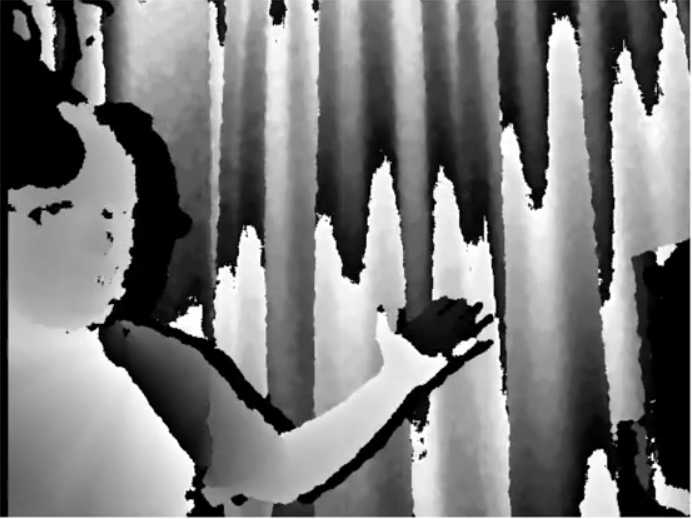
\includegraphics[scale=0.70]{./K1}}}%
    \qquad
    \subfloat[Kinect 2]{{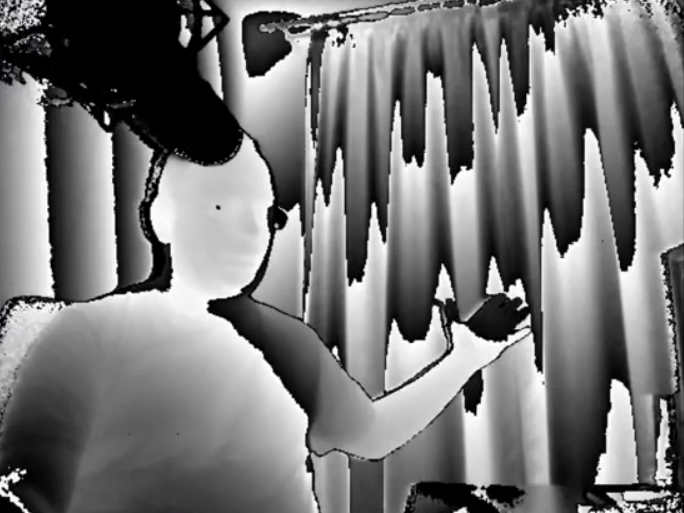
\includegraphics[scale=0.70]{./K2}}}%
    \caption{Kinect Output vs. Kinect 2 Output}
    \label{fig:KK2}
\end{figure}

We will explore Kinect 2 as a new sensor. If the extra resolution doesn't hit performance too hard, we will consider switching to it to be able to work with much cleaner data. 